\subsection{Calorimeter (CALO)}
\begin{figure}[h!]
\centering
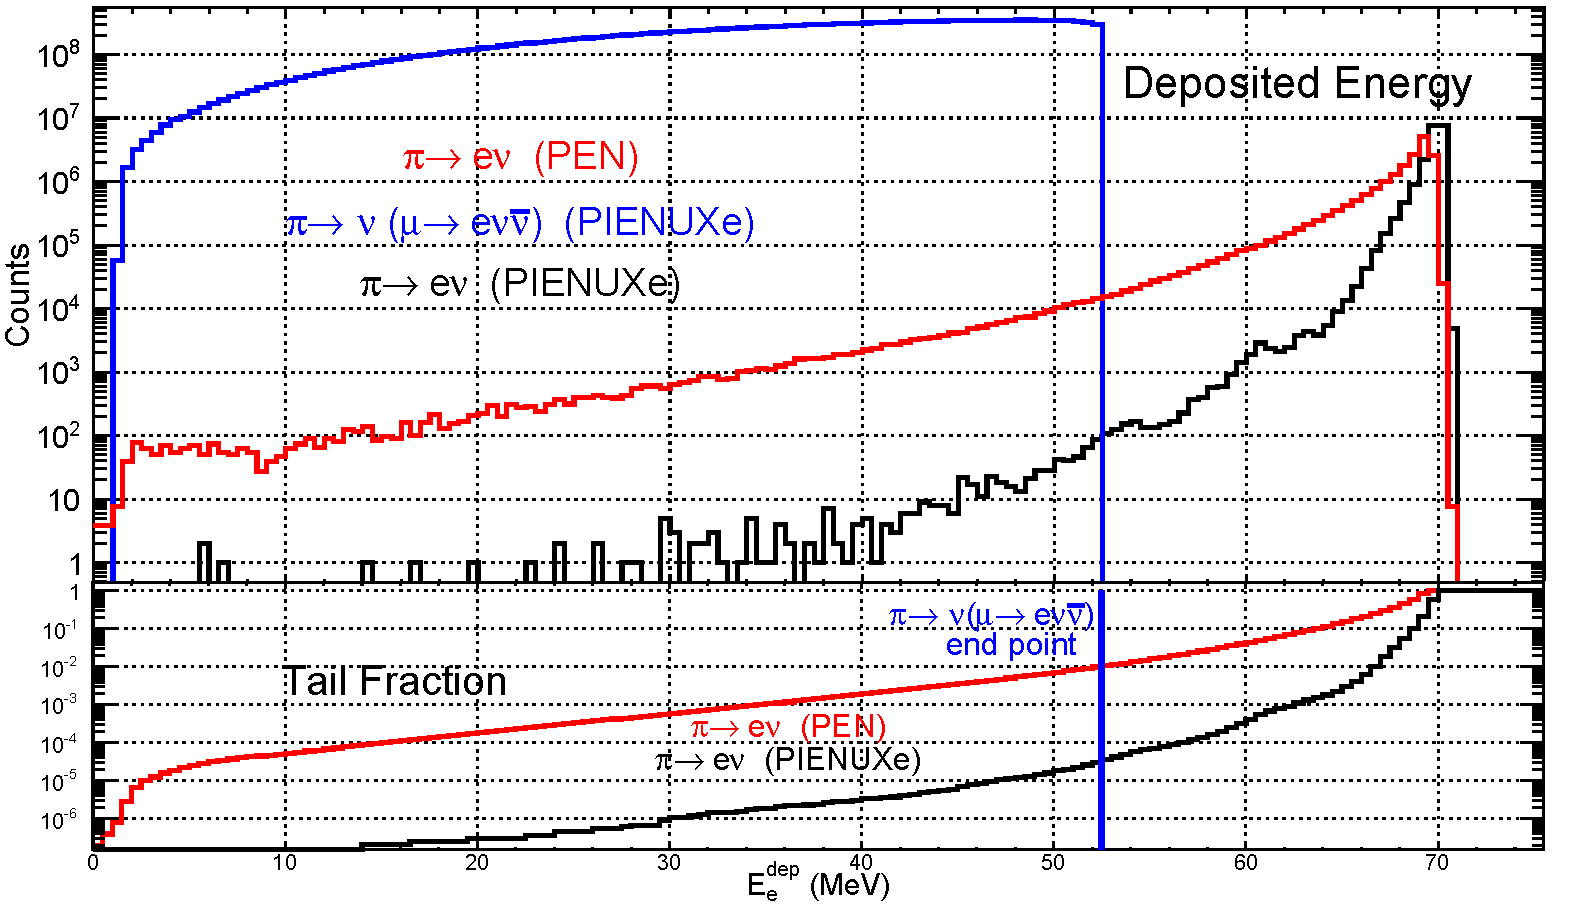
\includegraphics[scale=0.6]{sections/figures/tail.png}
\caption{Upper plot: histogram of $E_{e}^{dep}$, the $\pi_{e2}$ positron energy deposited in active components for a proposed 28 $X_{0}$ thick spherical LXe concept detector (black), compared with the same for the 12 $X_{0}$ pure CsI PEN apparatus (red), along with energy deposition
for the background $\pi \rightarrow \mu \rightarrow e$ decay chain events (blue).  Lower plot: comparison of the corresponding "tail" fractions as a function of $E_{e}^{dep}$; the LXe concept detector improves on the PEN fraction by two orders of magnitude in the region of interest.
\todo{I think we should add a PIENU spectrum as well and change the text accordingly}}
\label{fig:tail}
\end{figure}


A calorimeter covering 3$\pi$ solid angle with a thickness of 28 $X_0$ could dramatically reduce the ``tail” region
%-of-interest, 
which overlaps with the Michel spectrum, a key source of systematic uncertainty, see fig.\cite{fig:tail}. 
Two scintillation calorimeter options are presently under consideration: Liquid xenon and LSO crystals. Their main properties are compared in 
Table~\ref{tab:calos}. Evaluations  of potential energy and timing performance, rate capabilities, mechanical and cryogenic facilities, and cost are ongoing.
\begin{table}
\center
\begin{tabular}{cccccccc}
\hline
\hline
 detector 	&  density 		& 	dE/dx	&	$X_0$ 	& 	$R_M$ 	& decay time 	& $\lambda_{max}$ 	& light output  \\
 			&	g/cm3		&	MeV/cm	&	cm		&	cm		&	ns			&	nm				&	\%		\\	
\hline
LXe			&	2.953 		&	3.707	&	2.872	&	5.224	&	3, 27, 45	&	178			&	125 ?  \\
LSO(Ce)		&	7.40			&	9.6		&	1.14	&	2.07	&	40		&	402			&	85		\\	
\hline
\hline
\end{tabular}
\caption{LXe and LSO properties: density, minimum ioization, radiation length, Moli\`ere radius, decay times, maximum emission wavelength and relative light output compared to NaI(Tl). The LXe boiling point at 1 atm is 165.1 K. \todo{please check, LXe light output?}}
\label{tab:calos}
\end{table}


\subsubsection{LXe Calorimenter}
\begin{figure}[h!]
\centering
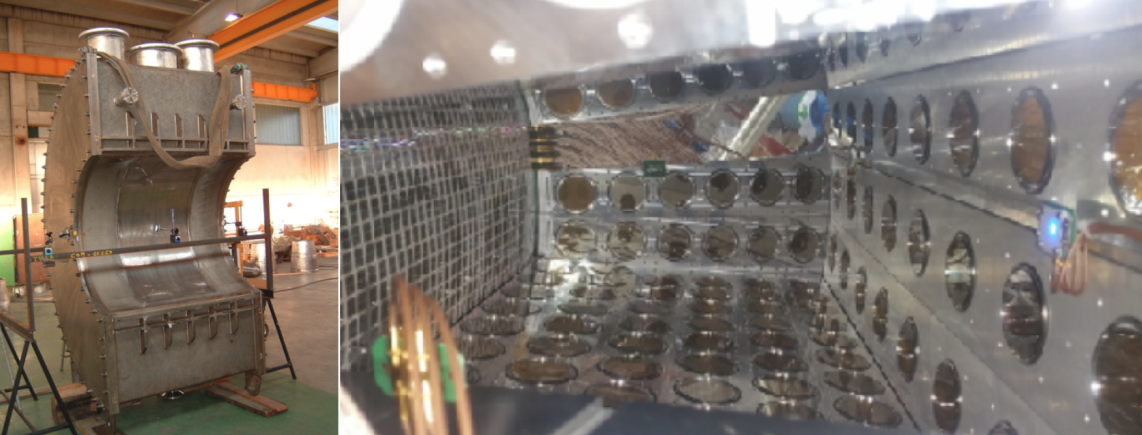
\includegraphics[scale=.4]{sections/figures/calo.meg.png}\vspace{3mm}\\
\caption{placeholder MEG, Toshiyuki please provide nice pictures}
\label{fig:calo.meg}
\end{figure}

One  concept for the new experiment is based on a liquid xenon (LXe) scintillating calorimeter for detection of positrons and gammas from pion decays. A 25-30 X$_o$ thick LXe scintillation calorimeter read out with fast-digitized SiPMs
has extraordinary properties including high light output (65k photons per MeV deposit), fast timing
($\sim$ ns decay time), and near complete containment of EM showers, making it suitable for this
application. Based on experience with the MEG LXe photon calorimeter \cite{Baldini} (see fig.~\cite{fig:calo.meg}) it is reasonable to
expect 1-2 \% energy resolution (comparable to \cite{Aguilar-Arevalo3} ), 50 ps timing resolution, and transverse (depth) position resolution of 5 mm 
(6 mm). Our Japanese collaborators are world experts on this detector technology. They have established basic LXe properties and suitable
simulation codes, conditioned on the MEG detector response, which will be critical for scaling up the design. \todo{Toshiyuki, Toshi, Sathoshi, that's just a placeholder for your part}
Due to the fast scintillation response of LXe (orders of magnitude faster than the NaI(Tl) and
pure CsI used in \cite{Aguilar-Arevalo1, Aguilar-Arevalo2} and \cite{Pocanic1, Pocanic2}), a low-energy pion beam rate of several 10$^5$ Hz can be used, more than an order of magnitude greater than previous experiments, which were impacted by pulse pile-up effects. Systematic effects would be reduced due to the highly uniform response and depth of the total absorption LXe calorimeter. 

\begin{figure}[h!]
\centering
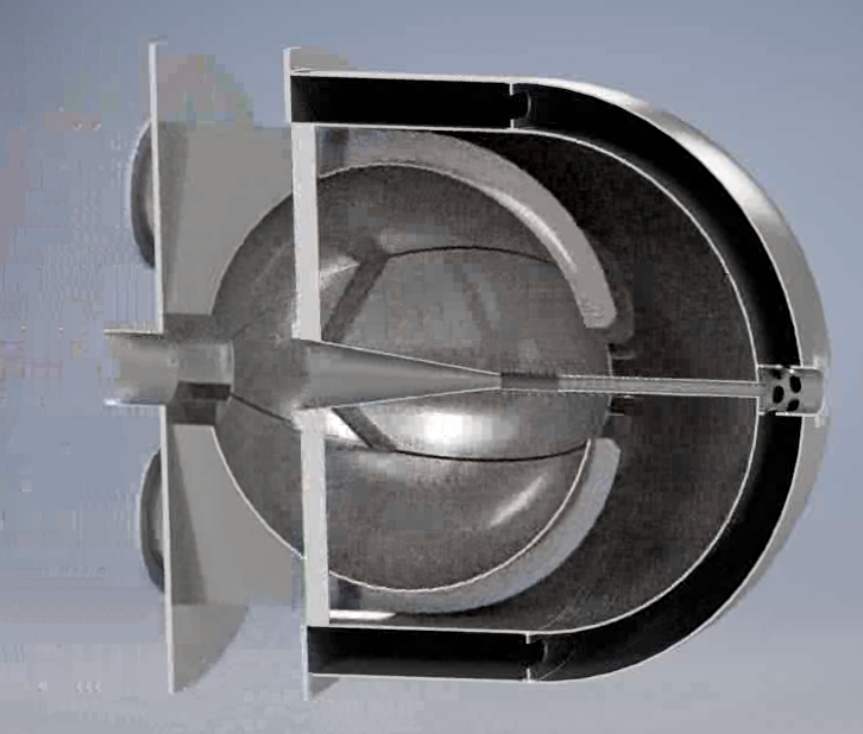
\includegraphics[scale=.4]{sections/figures/calo.Xe.png}
\caption{placeholder  \nexp\ CALO }
\label{fig:calo.Xe}
\end{figure}

\begin{table}
\center
\begin{tabular}{llll}
\hline
\hline
 parameter  &  	value		& 	unit		&  comment \\
\hline
Xe shell radius				&		&		&		\\
Xe volume					&		&		&		\\
Xe weight					&		&		&		\\
Xe entrance window radius	&		&		&		\\
vacuum window radius		&		&		&		\\
\hline
SiPM sensor size			&		&		&		\\
\# sensors					&		&		&		\\
\hline
\hline
\end{tabular}
\caption{Basic \nexp\ CALO parameters. \todo{Xe Ryan, SiPM Toshi, Satoshi et al}}
\label{tab:detpar}
\end{table}
The current conceptional design of the \nexp\ CALO draws on the experience of MEG, but involves several new features, see fig.~\ref{fig:calo.Xe} and Table~\ref{tab:detpar}.
\todo{Ryan: please continue}




\subsubsection{Crystal Calorimeter}


Another calorimeter concept is based on using LSO or LYSO crystals in a $3 \pi$ solid angle configuration similar to the PEN experiment discussed above. LSO has similar timing parameters to pure CsI (fast component aobut 45 ns) but much higher ligt output i.e. 75$\%$ of NaI(Tl). With a short radiation lenght about 1.1 cm, a compact calorimeter of 25-30 $X_0$ with excellent energy and time resolutions could be constructed. The same energy tail suppression would be realized as discussed above for the LXe option. The potential advantages of the crystal calorimeter approach include the absence of cryogenics and dead material, simpler mechanical facilities, and natural segmentation for handling high rates.